%%%%%%%%%%%%%%%%%%%%%%%%%%%%%%%%%%%%%%%%%%%%%%%%%%%%%%%%%%%%%%%%%%%%%%%%%%%%%%%%
\chapter{Разработка генератора систем инструментирования}
%%%%%%%%%%%%%%%%%%%%%%%%%%%%%%%%%%%%%%%%%%%%%%%%%%%%%%%%%%%%%%%%%%%%%%%%%%%%%%%%

Креатив.

%%%%%%%%%%%%%%%%%%%%%%%%%%%%%%%%%%%%%%%%%%%%%%%%%%%%%%%%%%%%%%%%%%%%%%%%%%%%%%%%
\section{Принцип работы системы инструментирования}
%%%%%%%%%%%%%%%%%%%%%%%%%%%%%%%%%%%%%%%%%%%%%%%%%%%%%%%%%%%%%%%%%%%%%%%%%%%%%%%%

***
Ключевыми идеями системы являются:
\begin{itemize}[noitemsep]
  \item Оперирование контекстами инструментирования как некоторыми множествами.
  \item Использование одного прохода по дереву разбора для осуществления требуемых манипуляций (вставки фрагментов программного кода).
\end{itemize}

%%%%%%%%%%%%%%%%%%%
\subsection{Взаимодействие с окружением}
%%%%%%%%%%%%%%%%%%%

***

На рис.~\ref{fig:layout_artefacts} приведена обобщенная схема работы системы с позиции обрабатываемых и производимых артефактов, таких как файлы и аргументы командной строки (параметры запуска).

\begin{figure}[!h]
	\centering
	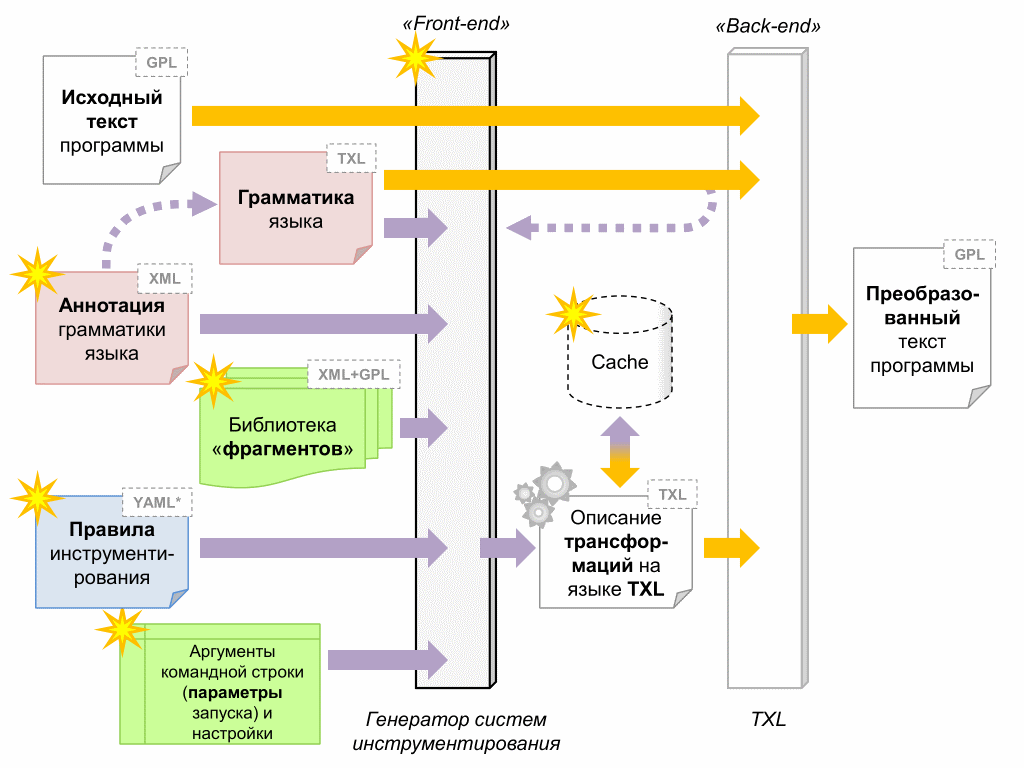
\includegraphics[width=4.2in]{layout_artefacts}
	\caption{Cхема работы системы. Артефакты.}
	\label{fig:layout_artefacts}
\end{figure}

для её работы необходимы:
\begin{itemize}[noitemsep]
  \item текст программы, инструментирование которой необходимо выполнить;
  \item описание грамматики языка, на котором написан исходный текст этой программы;
  \item аннотация грамматики языка;
  \item пользовательские правила инструментирования;
  \item фрагменты исходных текстов на выбранном языке программирования, вставку которых необбходимо выполнить;
  \item дополнительные необязательные параметры запуска системы и переменные среды исполнения.
\end{itemize}

***

%%%%%%%%%%%%%%%%%%%
\subsection{Правила инструментирования}
%%%%%%%%%%%%%%%%%%%

***
про язык

Декларативный язык.

***

Разработанный язык описания пользовательских правил долен в том или ином виде включать:

\begin{itemize}[noitemsep]
  \item перечисление интересующих пользователя контекстов инструментирования;
  \item перечисление используемых в данном наборе правил фрагментов исходных текстов, с указанием параметров, если таковые требуются согласно тексту используемого фрагмента;
  \item описывать уточнение контекста инструментирования с применением ключевых слов языка программирования и текстовых шаблонов, если таковые требуются для целей уточнения контекста согласно решаемой пользователем задачи;
  \item указание конкретной точки инструментирования каким-либо способом;
  \item объявление пользовательских переменных;
  \item поддерживать именование правил инструментирования.
\end{itemize}

%%%%%%%%%%%%%%%%%%%
\subsection{Аннотация грамматики языка}
%%%%%%%%%%%%%%%%%%%

***
про XML

Аннотация грамматики предназначается для сокращения множества $G$ всех узлов бесконечного множества деревьев разбора, описываемых грамматикой целевого языка программирования в виде графовой структуры, в данном случае -- с помощью языка утилиты TXL, до множества транзитивно связанных узлов $G^* \subset G$.

Одними из наиболее важных задач, решаемых составлением аннотации являются:

\begin{itemize}[noitemsep]
  \item описание всех синтаксических конструкций целевого языка программирования, наиболее существенных с точки зрения составителя аннотации, с учетом потребностей конечного пользователя в лице составителя правил инструментирования.
  \item описание всех точек инструментирования для всех выбранных синтаксических конструкций.
  \item императивное описание алгоритма инструментирования каждой точки инструментирования
\end{itemize}

Помимо этого, аннотация должна являться для пользователя упрощенной схемой иерархии типов узлов дерева разбора, в которой отображены только наиболее важные понятия языка программирования, для которого выполняется инструментирование, такие как \textit{класс}, \textit{метод}, \textit{оператор ветвления}, \textit{цикл со счетчиком} и т.п.

Поскольку аннотации включают в себя
шаблоны выбранных синтаксических конструкций целевого языка программирования вместе с 
алгоритмами, императивно описывающими процесс инструментирования всех перечисленных точек инструментирования,
необходимо перечислить требования к языку, используемому для описания аннотаций:

\begin{itemize}[noitemsep]
  \item текстовый вид представления данных;
  \item поддержка иерархических структур;
  \item возможность использования любых символьных последовательностей, включая используемые самим языком описания, путем экранирования специальных символов;
  \item ***;
\end{itemize}

Приведенным выше требованиям соответствуют, например, такие языки как JSON и XML.
\nomenclature{JSON}{JavaScript Object Notation -- язык описания объектов языка JavaScript}
\nomenclature{XML}{eXtensible Markup Language -- расширяемый язык разметки}

***

%%%%%%%%%%%%%%%%%%%
\subsection{Фрагменты программного кода}
%%%%%%%%%%%%%%%%%%%

***
про XML

***

%%%%%%%%%%%%%%%%%%%
\subsection{Пользователи системы}
%%%%%%%%%%%%%%%%%%%

На рис.~\ref{fig:layout_users} приведена схема работы системы инструментирования с позиции взаимодействия пользователей и системы как части производственного процесса (создания и отладки программного продукта).

\begin{figure}[h]
	\centering
	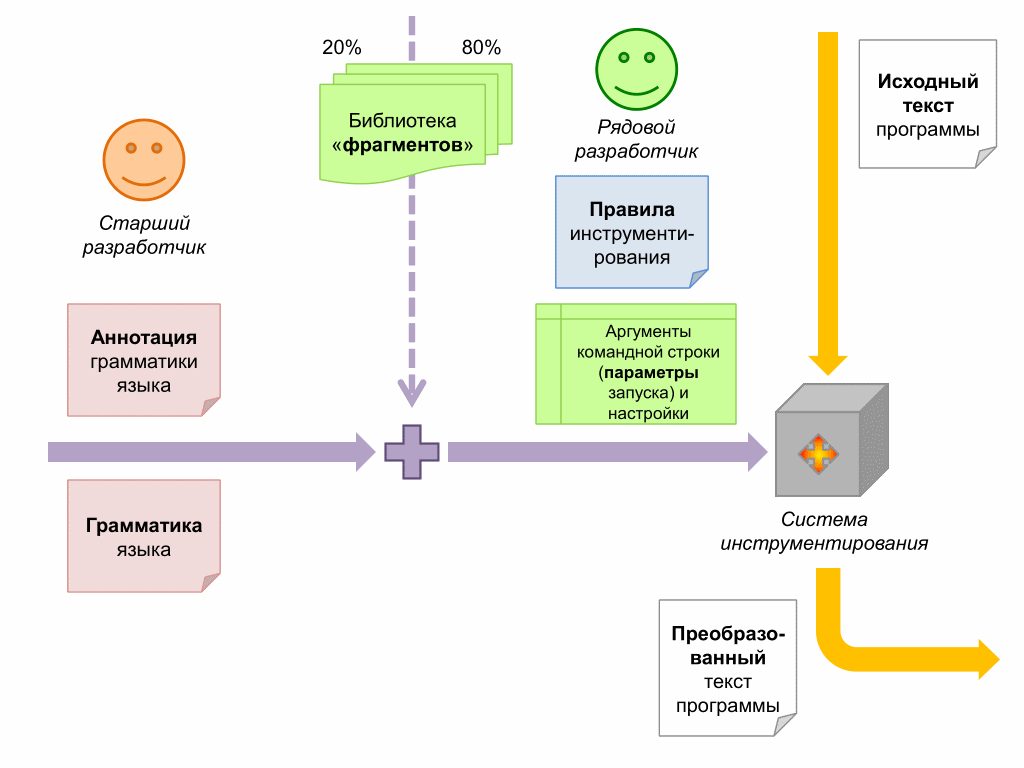
\includegraphics[width=4.2in]{layout_users}
	\caption{Cхема работы системы. Пользователи.}
	\label{fig:layout_users}
\end{figure}

***
с точки зрения пользователей есть два пользователя:

\begin{itemize}[noitemsep]
  \item Разработчик грамматики -- более опытный пользователь, в лице старшего разработчика, в задачи которого входит:
    \begin{itemize}[noitemsep]
      \item описание грамматики целевого языка программирования;
      \item составление аннотации к грамматике;
      \item отладка аннотации и грамматики;
      \item составление примеров фрагментов на целевом языке программирования.
    \end{itemize}

  \item Составитель правил инструментирования -- конечный пользователь, в лице рядового разработчика, в задачи которого входит:
    \begin{itemize}[noitemsep]
      \item составление правил инструментирования;
      \item создание и пополнение библиотеки фрагментов исходных текстов на целевом языке;
      \item применение системы инструментирования к исходным текстам какой-либо программной системы.
    \end{itemize}
\end{itemize}

Исходя из задач, решаемых разными пользователями системы, можно выделить следующий минимальный набор компетенций для разных групп пользователей системы:
\begin{itemize}[noitemsep]
  \item Разработчик грамматики:
    \begin{itemize}[noitemsep]
      \item 1
      \item 2
    \end{itemize}

  \item Составитель правил инструментирования:
    \begin{itemize}[noitemsep]
      \item 1
      \item 2
    \end{itemize}
\end{itemize}


%%%%%%%%%%%%%%%%%%%
\subsection{Выходные артефакты генератора}
%%%%%%%%%%%%%%%%%%%

***
про кэш и откат/копирование при ошибках

Исходя из предположения об использовании рассматриваемого генератора систем инструментирования как части процесса сборки некоторого промышленного программного обеспечения, которое имеет большой объем кодовой базы, можно сделать вывод о необходимости обеспечить разумный уровень сокращения повторяющихся ресурсо-затратных действий.

Наиболее ресурсо-затратными действиями при работе системы инструментирования будут следующие:
\begin{itemize}[noitemsep]
  \item чтение каких-либо данных из файлового хранилища (жесткие диски, RAID-массивы жестких дисков);
  \item запись каких-либо данных в файловое хранилище;
  \item анализ и предобработка считанных данных;
  \item обработка и синтез выходных данных во временной памяти;
  \item запуск и ожидание других процессов операционной системы.
\end{itemize}
\nomenclature{RAID}{Redundant Array of Independent Disks -- технология виртуализации данных для объединения физических дисковых устройств}

С учетом относительного времени, которое необходимо для выполнения различных операций, приведенный список можно упорядочить следующим образом (меньше номер -- лучше):
\begin{enumerate}[noitemsep]
  \item обработка и синтез выходных данных во временной памяти;
  \item анализ и предобработка считанных данных;
  \item чтение данных из файлового хранилища;
  \item запись данных в файловое хранилище;
  \item запуск и ожидание других процессов.
\end{enumerate}

Для простоты, примем время работы пунктов $1$ и $2$ одинаковым.

С учетом полученных результатов, рассмотрим более детально предполагаемый процесс инструментирования, изображенный на рисунке~\ref{fig:layout_artefacts}, уделяя внимание наиболее ресурсоемким выполняемым операциям.

Для генерации промежуточного описания трансформаций на языке TXL, генератору требуется выполнить \textbf{чтение} из файлового хранилища следующих артефактов:
\begin{itemize}[noitemsep]
  \item грамматика целевого языка программирования;
  \item аннотация к грамматике;
  \item пользовательские правила инструментирования;
  \item несколько фрагментов из библиотеки фрагментов (зависимость от пользовательского описания, $N$).
\end{itemize}

Таким образом, генератор систем инструментирования должен выполнить $3 + N$ раздельных чтений из файлового хранилища, чтобы впоследствии выполнить \textbf{запись} в файловое хранилище промежуточного описания трансформаций и \textbf{запустить} утилиту TXL, которая в свою очередь выполнит несколько (минимум $3$, как видно на рис.~\ref{fig:layout_artefacts}) чтений и, как минимум, одну запись, в зависимости от сложности и структуры грамматики целевого языка программирования, для непосредственного инструментирования обрабатываемого исходного текста программы как часть завершающего этапа.

Исходя из специфики решаемой задачи, работы завершающего этапа необходимо выполнять для каждого файла исходного текста на целевом языке, содержащимся в кодовой базе инструментируемого ПО.
Таким образом, для оценки множества ресурсо-затратных действий, выполняемых системой инструментирования (генератор и утилита TXL), необходимо исключить из рассмотрения действия, выполняемые утилитой TXL, т.е. действия завершающего этапа инструментирования.

Помимо работы с файловым хранилищем, система инструментирования, в часности генератор, выполняет разбор и анализ загруженных данных, после чего обработку и синтез промежуточного описания правил трансформаций.
Перечисленные операции (разбор, анализ, обработка, синтез) производятся во временной памяти.

Следуя заключениям выше, составим общий объем работ, выполняемый ***

***

%%%%%%%%%%%%%%%%%%%
\section{Задача инструментирования}
%%%%%%%%%%%%%%%%%%%

***

%%%%%%%%%
\subsection{Обработка деревьев разбора}
%%%%%%%%%

***

Способы обхода древовидных структур данных:
* обход вглубину
* обход вширину

Исходя из функциональной природы языка TXL, *

***

Приведенные выше рассуждения приводят к формулировке метода, который способен решить поставленную задачу.

***

%%%%%
\subsubsection{Нисходящий однопроходный метод}
%%%%%

Основная идея -- спуск по дереву разбора (CST) от корневого узла к листьям, собирая по пути следования информацию для определения контекста, в котором находятся обрабатываемые/инструментируемые узлы.
\nomenclature{CST}{Concrete Syntax Tree -- конкретное дерево разбора}

Обход "в глубину" (DFT).
\nomenclature{DFT}{Depth-First Traversal -- метод обхода графовой структуры, состоящий в том, чтобы идти ``вглубь'' графа, насколько это возможно}

***

Основная идея нисходящего подхода заключается в постепенном спуске по дереву разбора, которое генерирует внутри себя утилита TXL, от корневого узла к листьям, сохраняя по пути следования информацию для определения контекста, в котором находятся обрабатываемые узлы и выполняется инструментирование.

Данный метод хорошо соотносится с функциональной природой языка TXL, с помощью которого можно описать цепочку вызовов взаимосвязанных функций для обработки различных вложенных типов узлов дерева разбора.

Однако, данный метод подходит только для таких языков программирования, которые соответствуют принципу вложенности синтаксических элементов, т.е. программы, составленные на данных языках программирования соответствуют \textit{структурной парадигме} программирования [***].

***

%%%%%
\subsubsection{Нисходящий многопроходный метод}
%%%%%

***

%%%%%%%%%
\subsection{Контексты инструментирования}
%%%%%%%%%

иснтрументирование подразумевает использование некоторых контекстов, поэтому с ними было бы удобно работать как с множествами

Проблема представления деревьев в виде множеств
Или сопоставления деревьев и множеств
правила грамматики могут описывать бесконечные деревья

\begin{figure}[H]
	\centering
	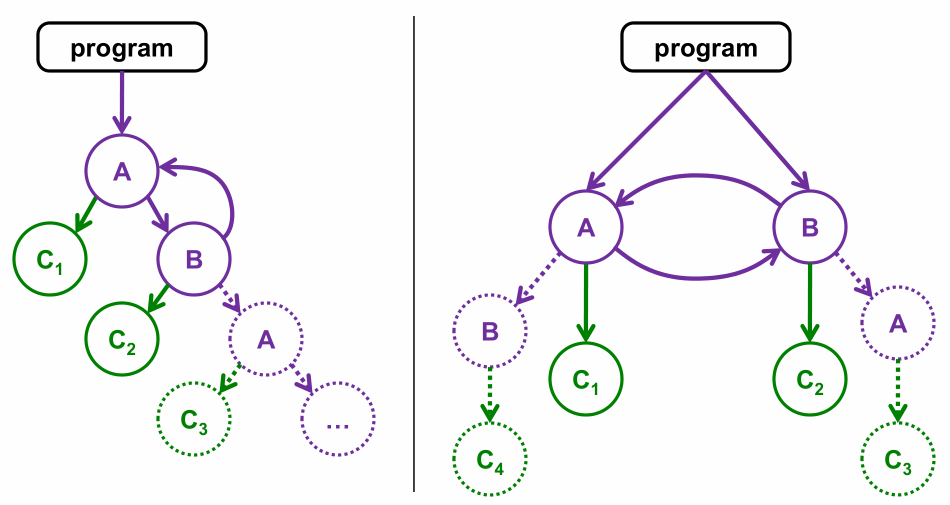
\includegraphics[width=3.2in]{tree_inf}
	\caption{Пример дерева разбора с повторением типов узлов}
	\label{fig:tree_inf}
\end{figure}

рассмотрим пример: пусть $A$, $B$, $C$, $D$ -- ***

какие есть способы описания ограничений в TXL
один из них -- КНФ

исходя из этого
$A * B + C * D$
переходит в
$(A + C) * (A + D) * (B + C) * (B + D)$

***

Поскольку язык, который используется для программирования утилиты TXL, принадлежит к семейству функциональных языков программирования, это ограничение заставляет передавать собираемую информацию посредством аргументов/параметров, с которыми вызываются последующие функции в цепочке.

***

теперь необходимо распределить эти ограничения по функциям в соответствии с узлами из дерева рабора, которые содержат значения, которые нужно проверить

***

\begin{figure}[H]
	\centering
	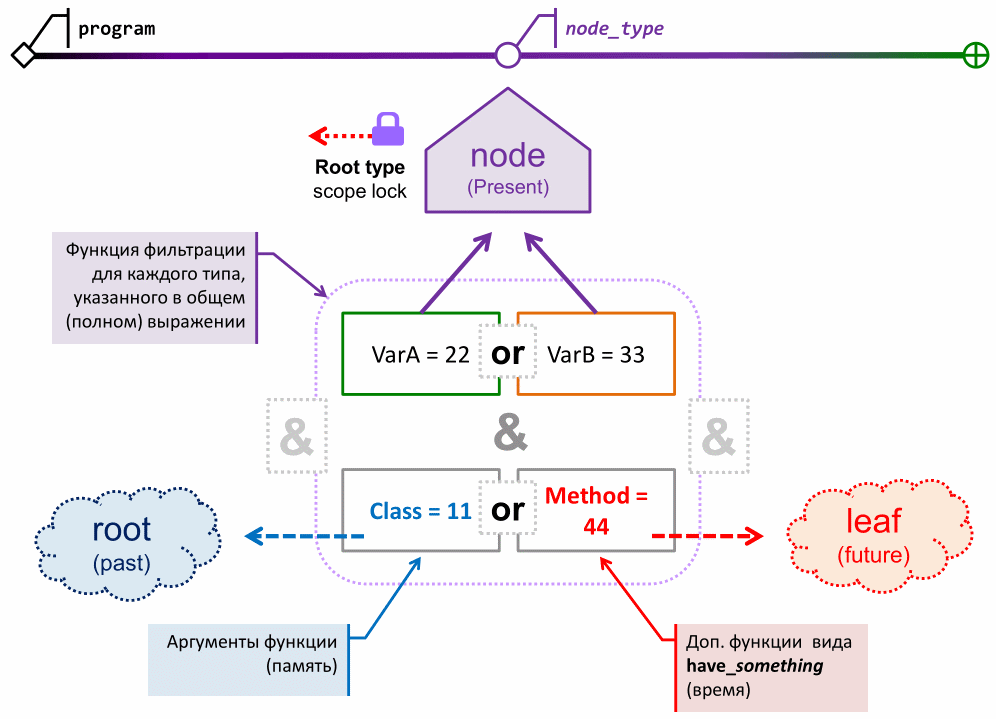
\includegraphics[width=3.5in]{filter_abstract}
	\caption{Обобщенная модель функции фильтрации по контексту инструментирования.}
	\label{fig:filter_abstract}
\end{figure}

***

Группировка по типам узлов дерева разбора, которые содержат данные, на основе которых выполняется принятие решения о принадлежности к контексту инструментирования. Иными словами -- содержат значения, проверяемые ограничениями из формул.

\begin{figure}[H]
	\centering
	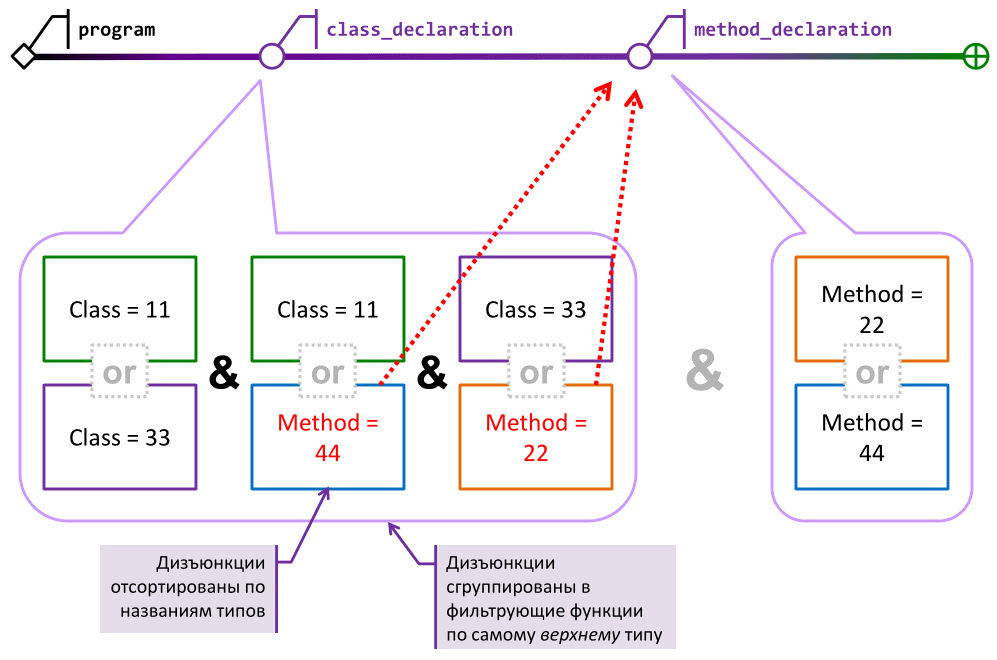
\includegraphics[width=3.2in]{filter_types}
	\caption{Группировка ограничений. По типам узлов.}
	\label{fig:filter_types}
\end{figure}

***

Группировка с применением дополнительных функций сбора информации.

\begin{figure}[H]
	\centering
	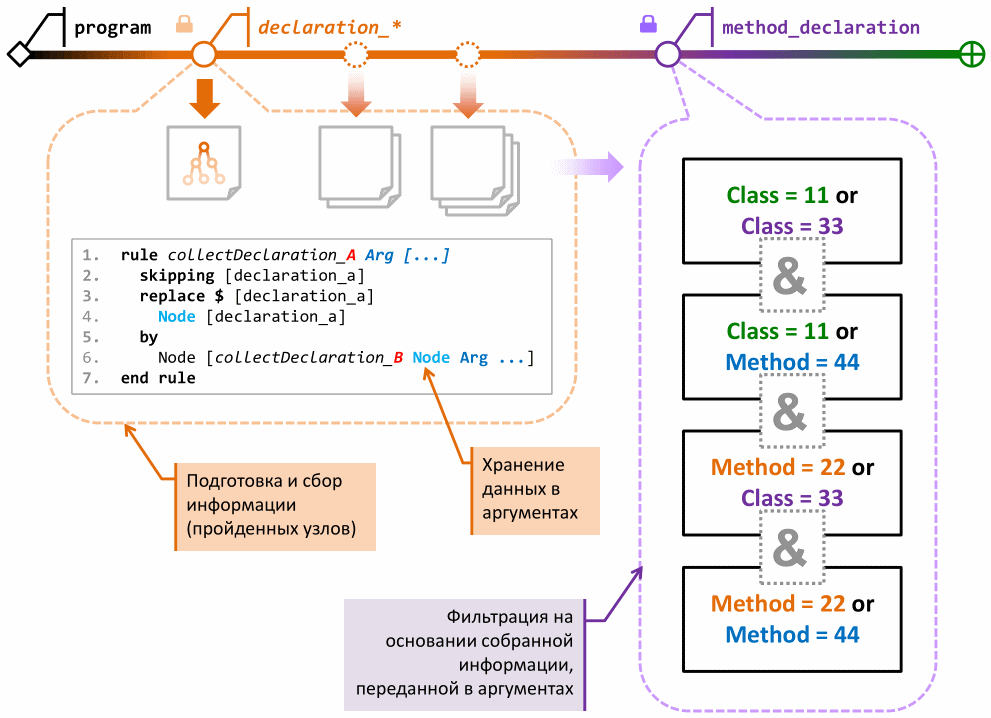
\includegraphics[width=3.7in]{filter_collect}
	\caption{Группировка ограничений. Дополнительные функции.}
	\label{fig:filter_collect}
\end{figure}

***

%%%%%%%%%%%%%%%%%%%%%%%%%%%%%%%%%%%%%%%%%%%%%%%%%%%%%%%%%%%%%%%%%%%%%%%%%%%%%%%%
\section{Выводы}
%%%%%%%%%%%%%%%%%%%%%%%%%%%%%%%%%%%%%%%%%%%%%%%%%%%%%%%%%%%%%%%%%%%%%%%%%%%%%%%%

Текст.
